%---------------
%╔═╗╔═╗╔╦╗╦ ╦╔═╗
%╚═╗║╣  ║ ║ ║╠═╝
%╚═╝╚═╝ ╩ ╚═╝╩  
%---------------
\documentclass[12pt,oneside,a4paper]{report}

% DOCUMENT SETUP
\usepackage[left=3cm, 
			right=2.5cm, 
			top=2.5cm, 
			bottom=2.5cm, 
			includehead, 
			includefoot]{geometry}

% line spacing
\usepackage{setspace}
\setstretch{1,25} % 15/12 --> 1.25

%de­fines Adobe Times Ro­man as de­fault text font
\usepackage{mathptmx}
\usepackage{times} % needed for acronym package

%PDF linking package
\usepackage[hidelinks]{hyperref}

% Language Setup
\usepackage[ngerman]{babel}
% language specific bibliography style
\usepackage[numbers]{natbib}
\usepackage[fixlanguage]{babelbib}
\selectbiblanguage{german}
% bliographystyle setup
% default style names: apalike alphadin ieeetr IEEEtranSN apalike2 alphadin 
% babel specific: babplain, babplai3, babalpha, babunsrt, bababbrv, bababbr3 unsrt 
\bibliographystyle{unsrturl}

% encoding setup
% T1 font encoding for languages that use a latin alphabet
\usepackage[T1]{fontenc} 

% enhanced input encoding handling - utf8 for äÄüÜöÖß...
\usepackage[utf8]{inputenc}
%\usepackage{ucs}%utf8x suppart

% after babel - set chapter string
\AtBeginDocument{\renewcommand{\chaptername}{}}

% enumeration
\usepackage{enumitem}
% tabular extension tabularx
\usepackage{tabularx}

% math packages
\usepackage{amsmath}
\usepackage{nicefrac}
\usepackage{amsthm}
\usepackage{amsbsy}
\usepackage{amssymb}
\usepackage{amsfonts}
\usepackage{MnSymbol}

% patches for latex
\usepackage{fixltx2e}

%special characters
\usepackage{amssymb}
\usepackage{upgreek,textgreek}

% acronym package
\usepackage[printonlyused, footnote]{acronym}

% breakable text in \seqsplit{}
\usepackage{seqsplit}

% \textmu
\usepackage{textcomp}

% package provides a way to compile sections of a document using the same preamble as the main document
\usepackage{subfiles}

% driver-independent color extension - used by listings,tabularx
\usepackage[usenames,dvipsnames,table,xcdraw]{xcolor}

% -- SYNTAX HIGHLIGHTING --
\usepackage{listings}
%% bash command line Syntax Highlighting
\lstdefinestyle{BASH_CMD}{ 
  columns=fullflexible,            % copy pasteable listings
  language=bash,
  basicstyle=\small\sffamily,
  basicstyle   = \small \ttfamily,
  keywordstyle = [1]\small \ttfamily,
  keywordstyle = [2]\small \ttfamily,
  commentstyle = \small \ttfamily,
  numbers=none,
  captionpos=b, 
  breaklines=true,
  numberstyle=\tiny,
  numbersep=3pt,
  frame=tlrb,
  columns=fullflexible,
  backgroundcolor=\color{white!20},
  linewidth=\linewidth,
  literate=                        % replace in code
     {Ö}{{\"O}}1
     {Ä}{{\"A}}1
     {Ü}{{\"U}}1
     {ß}{{\ss}}2
     {ü}{{\"u}}1
     {ä}{{\"a}}1
     {ö}{{\"o}}1
}
 % adds style BASH_CMD
%% Matlab Syntax Highlighting
\colorlet{keyword}{blue!100!black!80}
\colorlet{STD}{Lavender}
\colorlet{comment}{green!90!black!90}
\definecolor{mygreen}{rgb}{0,0.6,0}
\definecolor{mygray}{rgb}{0.5,0.5,0.5}
\definecolor{mymauve}{rgb}{0.58,0,0.82}


\lstdefinestyle{BASH_SCRIPT}{ 
  language     = bash,
  basicstyle   = \footnotesize \ttfamily,
  keywordstyle = [1]\color{keyword}\bfseries,
  keywordstyle = [2]\color{STD}\bfseries,
  commentstyle = \color{mygreen}\itshape,
  backgroundcolor=\color{white},   % choose the background color; you must add \usepackage{color} 
  columns=fullflexible,            % copy pasteable listings
                                   % or \usepackage{xcolor}
  basicstyle=\footnotesize,        % the size of the fonts that are used for the code
  breakatwhitespace=false,         % sets if automatic breaks should only happen at whitespace
  breaklines=true,                 % sets automatic line breaking
  captionpos=b,                    % sets the caption-position to bottom
  extendedchars=true,              % lets you use non-ASCII characters; for 8-bits encodings only,
                                   % does not work with UTF-8
  frame=single,                    % adds a frame around the code
  keepspaces=true,                 % keeps spaces in text, useful for keeping indentation of code
                                   % (possibly needs columns=flexible)
  numbers=left,                    % where to put the line-numbers; possible values are 
                                   % (none, left, right)
  numbersep=5pt,                   % how far the line-numbers are from the code
  numberstyle=\tiny\color{mygray}, % the style that is used for the line-numbers
  rulecolor=\color{black},         % if not set, the frame-color may be changed on line-breaks
                                   % within not-black text (e.g. comments (green here))
  showspaces=false,                % show spaces everywhere adding particular underscores; it
  	                               % overrides 'showstringspaces'
  showstringspaces=false,          % underline spaces within strings only
  showtabs=false,                  % show tabs within strings adding particular underscores
  stepnumber=1,                    % the step between two line-numbers. If it's 1, each line 
                                   % will be numbered
  stringstyle=\color{mymauve},     % string literal style
  tabsize=2,                       % sets default tabsize to 2 spaces
  title=\lstname,                  % set title name
  literate=                        % replace in code
     {Ö}{{\"O}}1
     {Ä}{{\"A}}1
     {Ü}{{\"U}}1
     {ß}{{\ss}}2
     {ü}{{\"u}}1
     {ä}{{\"a}}1
     {ö}{{\"o}}1
} % adds style BASH_SCRIPT
% Matlab Syntax Highlighting
\colorlet{keyword}{blue!100!black!80}
\colorlet{STD}{red}
\colorlet{comment}{green!90!black!90}
\definecolor{mygreen}{rgb}{0,0.6,0}
\definecolor{mygray}{rgb}{0.5,0.5,0.5}
\definecolor{mymauve}{rgb}{0.58,0,0.82}


\lstdefinestyle{LATEX}{ 
  language     = [LaTeX]{TeX},
  basicstyle   = \footnotesize \ttfamily,
  keywordstyle = [1]\color{keyword}\bfseries,
  keywordstyle = [2]\color{comment}\bfseries,
  commentstyle = \color{mygray}\itshape,
  %backgroundcolor=\color{white},   % choose the background color; you must add \usepackage{color} 
                                   % or \usepackage{xcolor}
  basicstyle=\footnotesize,        		   % the size of the fonts that are used for the code
  breakatwhitespace=false,         % sets if automatic breaks should only happen at whitespace
  columns=fullflexible,            % copy pasteable listings
  breaklines=true,                 % sets automatic line breaking
  captionpos=c,                    % sets the caption-position to bottom
  extendedchars=true,              % lets you use non-ASCII characters; for 8-bits encodings only,
                                   % does not work with UTF-8
  frame=single,                    % adds a frame around the code
  keepspaces=true,                 % keeps spaces in text, useful for keeping indentation of code
                                   % (possibly needs columns=flexible)
  numbers=left,                    % where to put the line-numbers; possible values are 
                                   % (none, left, right)
  numbersep=4pt,                   % how far the line-numbers are from the code
  numberstyle=\tiny\color{mygray}, % the style that is used for the line-numbers
  rulecolor=\color{black},         % if not set, the frame-color may be changed on line-breaks
                                   % within not-black text (e.g. comments (green here))
  showspaces=false,                % show spaces everywhere adding particular underscores; it
  	                               % overrides 'showstringspaces'
  showstringspaces=false,          % underline spaces within strings only
  showtabs=false,                  % show tabs within strings adding particular underscores
  stepnumber=1,                    % the step between two line-numbers. If it's 1, each line 
                                   % will be numbered
  stringstyle=\color{mymauve},     % string literal style
  tabsize=2,                       % sets default tabsize to 2 spaces
  title=\lstname,                  % set title name
  literate=                        % replace in code
     {Ö}{{\"O}}1
     {Ä}{{\"A}}1
     {Ü}{{\"U}}1
     {ß}{{\ss}}2
     {ü}{{\"u}}1
     {ä}{{\"a}}1
     {ö}{{\"o}}1
} % adds style LATEX
%% Matlab Syntax Highlighting
\colorlet{keyword}{blue!100!black!80}
\colorlet{STD}{Lavender}
\colorlet{comment}{green!90!black!90}
\definecolor{mygreen}{rgb}{0,0.6,0}
\definecolor{mygray}{rgb}{0.5,0.5,0.5}
\definecolor{mymauve}{rgb}{0.58,0,0.82}


\lstdefinestyle{MATLAB}{ 
  language     = Matlab,
  basicstyle   = \footnotesize \ttfamily,
  keywordstyle = [1]\color{keyword}\bfseries,
  keywordstyle = [2]\color{STD}\bfseries,
  commentstyle = \color{mygreen}\itshape,
  backgroundcolor=\color{white},   % choose the background color; you must add \usepackage{color} 
                                   % or \usepackage{xcolor}
  basicstyle=\footnotesize,        % the size of the fonts that are used for the code
  breakatwhitespace=false,         % sets if automatic breaks should only happen at whitespace
  columns=fullflexible,            % copy pasteable listings
  breaklines=false,                % sets automatic line breaking
  captionpos=c,                    % sets the caption-position to bottom
  extendedchars=true,              % lets you use non-ASCII characters; for 8-bits encodings only,
                                   % does not work with UTF-8
  frame=single,                    % adds a frame around the code
  keepspaces=true,                 % keeps spaces in text, useful for keeping indentation of code
                                   % (possibly needs columns=flexible)
  numbers=left,                    % where to put the line-numbers; possible values are 
                                   % (none, left, right)
  numbersep=5pt,                   % how far the line-numbers are from the code
  numberstyle=\tiny\color{mygray}, % the style that is used for the line-numbers
  rulecolor=\color{black},         % if not set, the frame-color may be changed on line-breaks
                                   % within not-black text (e.g. comments (green here))
  showspaces=false,                % show spaces everywhere adding particular underscores; it
  	                               % overrides 'showstringspaces'
  showstringspaces=false,          % underline spaces within strings only
  showtabs=false,                  % show tabs within strings adding particular underscores
  stepnumber=1,                    % the step between two line-numbers. If it's 1, each line 
                                   % will be numbered
  stringstyle=\color{mymauve},     % string literal style
  tabsize=2,                       % sets default tabsize to 2 spaces
  title=\lstname,                  % set title name
  literate=                        % replace in code
     {Ö}{{\"O}}1
     {Ä}{{\"A}}1
     {Ü}{{\"U}}1
     {ß}{{\ss}}2
     {ü}{{\"u}}1
     {ä}{{\"a}}1
     {ö}{{\"o}}1
} % adds style MATLAB
% Matlab Syntax Highlighting
\colorlet{keyword}{blue!100!black!80}
\colorlet{STD}{Lavender}
\colorlet{comment}{green!90!black!90}
\definecolor{mygreen}{rgb}{0,0.6,0}
\definecolor{mygray}{rgb}{0.5,0.5,0.5}
\definecolor{mymauve}{rgb}{0.58,0,0.82}


\lstdefinestyle{PYTHON}{ 
  language     = Python,
  basicstyle   = \footnotesize \ttfamily,
  keywordstyle = [1]\color{keyword}\bfseries,
  keywordstyle = [2]\color{STD}\bfseries,
  commentstyle = \color{mygreen}\itshape,
  backgroundcolor=\color{white},   % choose the background color; you must add \usepackage{color} 
                                   % or \usepackage{xcolor}
  basicstyle=\footnotesize,        % the size of the fonts that are used for the code
  columns=fullflexible,            % copy pasteable listings
  breakatwhitespace=false,         % sets if automatic breaks should only happen at whitespace
  breaklines=false,                % sets automatic line breaking
  captionpos=c,                    % sets the caption-position to bottom
  extendedchars=true,              % lets you use non-ASCII characters; for 8-bits encodings only,
                                   % does not work with UTF-8
  frame=single,                    % adds a frame around the code
  keepspaces=true,                 % keeps spaces in text, useful for keeping indentation of code
                                   % (possibly needs columns=flexible)
  numbers=left,                    % where to put the line-numbers; possible values are 
                                   % (none, left, right)
  numbersep=5pt,                   % how far the line-numbers are from the code
  numberstyle=\tiny\color{mygray}, % the style that is used for the line-numbers
  rulecolor=\color{black},         % if not set, the frame-color may be changed on line-breaks
                                   % within not-black text (e.g. comments (green here))
  showspaces=false,                % show spaces everywhere adding particular underscores; it
  	                               % overrides 'showstringspaces'
  showstringspaces=false,          % underline spaces within strings only
  showtabs=false,                  % show tabs within strings adding particular underscores
  stepnumber=1,                    % the step between two line-numbers. If it's 1, each line 
                                   % will be numbered
  stringstyle=\color{mymauve},     % string literal style
  tabsize=2,                       % sets default tabsize to 2 spaces
  title=\lstname,                  % set title name
  literate=                        % replace in code
     {Ö}{{\"O}}1
     {Ä}{{\"A}}1
     {Ü}{{\"U}}1
     {ß}{{\ss}}2
     {ü}{{\"u}}1
     {ä}{{\"a}}1
     {ö}{{\"o}}1
} % adds style PYTHON
%% Matlab Syntax Highlighting
\colorlet{keyword}{blue!100!black!80}
\colorlet{STD}{Lavender}
\colorlet{comment}{green!90!black!90}
\definecolor{mygreen}{rgb}{0,0.6,0}
\definecolor{mygray}{rgb}{0.5,0.5,0.5}
\definecolor{mymauve}{rgb}{0.58,0,0.82}


\lstdefinestyle{CPP}{ 
  language     = C++,
  basicstyle   = \footnotesize \ttfamily,
  keywordstyle = [1]\color{keyword}\bfseries,
  keywordstyle = [2]\color{STD}\bfseries,
  commentstyle = \color{mygreen}\itshape,
  backgroundcolor=\color{white},   % choose the background color; you must add \usepackage{color} 
                                   % or \usepackage{xcolor}
  columns=fullflexible,            % copy pasteable listings
  basicstyle=\footnotesize,        % the size of the fonts that are used for the code
  breakatwhitespace=false,         % sets if automatic breaks should only happen at whitespace
  breaklines=false,                % sets automatic line breaking
  captionpos=c,                    % sets the caption-position to bottom
  extendedchars=true,              % lets you use non-ASCII characters; for 8-bits encodings only,
                                   % does not work with UTF-8
  frame=single,                    % adds a frame around the code
  keepspaces=true,                 % keeps spaces in text, useful for keeping indentation of code
                                   % (possibly needs columns=flexible)
  numbers=left,                    % where to put the line-numbers; possible values are 
                                   % (none, left, right)
  numbersep=5pt,                   % how far the line-numbers are from the code
  numberstyle=\tiny\color{mygray}, % the style that is used for the line-numbers
  rulecolor=\color{black},         % if not set, the frame-color may be changed on line-breaks
                                   % within not-black text (e.g. comments (green here))
  showspaces=false,                % show spaces everywhere adding particular underscores; it
  	                               % overrides 'showstringspaces'
  showstringspaces=false,          % underline spaces within strings only
  showtabs=false,                  % show tabs within strings adding particular underscores
  stepnumber=1,                    % the step between two line-numbers. If it's 1, each line 
                                   % will be numbered
  stringstyle=\color{mymauve},     % string literal style
  tabsize=2,                       % sets default tabsize to 2 spaces
  title=\lstname,                  % set title name
  literate=                        % replace in code
     {Ö}{{\"O}}1
     {Ä}{{\"A}}1
     {Ü}{{\"U}}1
     {ß}{{\ss}}2
     {ü}{{\"u}}1
     {ä}{{\"a}}1
     {ö}{{\"o}}1
} % adds style CPP
%% Matlab Syntax Highlighting
\colorlet{keyword}{blue!100!black!80}
\colorlet{STD}{Lavender}
\colorlet{comment}{green!90!black!90}
\definecolor{mygreen}{rgb}{0,0.6,0}
\definecolor{mygray}{rgb}{0.5,0.5,0.5}
\definecolor{mymauve}{rgb}{0.58,0,0.82}


\lstdefinestyle{C}{ 
  language     = C,
  basicstyle   = \footnotesize \ttfamily,
  keywordstyle = [1]\color{keyword}\bfseries,
  keywordstyle = [2]\color{STD}\bfseries,
  commentstyle = \color{mygreen}\itshape,
  backgroundcolor=\color{white},   % choose the background color; you must add \usepackage{color} 
  columns=fullflexible,            % copy pasteable listings
                                   % or \usepackage{xcolor}
  basicstyle=\footnotesize,        % the size of the fonts that are used for the code
  breakatwhitespace=false,         % sets if automatic breaks should only happen at whitespace
  breaklines=false,                % sets automatic line breaking
  captionpos=c,                    % sets the caption-position to bottom
  extendedchars=true,              % lets you use non-ASCII characters; for 8-bits encodings only,
                                   % does not work with UTF-8
  frame=single,                    % adds a frame around the code
  keepspaces=true,                 % keeps spaces in text, useful for keeping indentation of code
                                   % (possibly needs columns=flexible)
  numbers=left,                    % where to put the line-numbers; possible values are 
                                   % (none, left, right)
  numbersep=5pt,                   % how far the line-numbers are from the code
  numberstyle=\tiny\color{mygray}, % the style that is used for the line-numbers
  rulecolor=\color{black},         % if not set, the frame-color may be changed on line-breaks
                                   % within not-black text (e.g. comments (green here))
  showspaces=false,                % show spaces everywhere adding particular underscores; it
  	                               % overrides 'showstringspaces'
  showstringspaces=false,          % underline spaces within strings only
  showtabs=false,                  % show tabs within strings adding particular underscores
  stepnumber=1,                    % the step between two line-numbers. If it's 1, each line 
                                   % will be numbered
  stringstyle=\color{mymauve},     % string literal style
  tabsize=2,                       % sets default tabsize to 2 spaces
  title=\lstname,                  % set title name
  literate=                        % replace in code
     {Ö}{{\"O}}1
     {Ä}{{\"A}}1
     {Ü}{{\"U}}1
     {ß}{{\ss}}2
     {ü}{{\"u}}1
     {ä}{{\"a}}1
     {ö}{{\"o}}1
} % adds style C
%% JSON Syntax Highlighting
\colorlet{keyword}{blue!100!black!80}
\colorlet{STD}{Lavender}
\colorlet{comment}{green!90!black!90}
\definecolor{mygreen}{rgb}{0,0.6,0}
\definecolor{mygray}{rgb}{0.5,0.5,0.5}
\definecolor{mymauve}{rgb}{0.58,0,0.82}

\newcommand\JSONnumbervaluestyle{\color{blue}}
\newcommand\JSONstringvaluestyle{\color{red}}

\newif\ifcolonfoundonthisline

\makeatletter

\lstdefinelanguage{json}
{
  showstringspaces    = false,
  keywords            = {false,true},
  alsoletter          = 0123456789.,
  morestring          = [s]{"}{"},
  morestring          = [s]{'}{'},
  stringstyle         = \ifcolonfoundonthisline\JSONstringvaluestyle\fi,
  MoreSelectCharTable =%
    \lst@DefSaveDef{`:}\colon@json{\processColon@json},
  basicstyle          = \ttfamily,
  keywordstyle        = \ttfamily\bfseries,
}

% flip the switch if a colon is found in Pmode
\newcommand\processColon@json{
  \colon@json%
  \ifnum\lst@mode=\lst@Pmode%
    \global\colonfoundonthislinetrue%
  \fi
}

\lst@AddToHook{Output}{%
  \ifcolonfoundonthisline%
    \ifnum\lst@mode=\lst@Pmode%
      \def\lst@thestyle{\JSONnumbervaluestyle}%
    \fi
  \fi
  %override by keyword style if a keyword is detected!
  \lsthk@DetectKeywords% 
}

% reset the switch at the end of line
\lst@AddToHook{EOL}%
  {\global\colonfoundonthislinefalse}

\makeatother



\lstdefinestyle{JSON}{ 
  language     = json,
  basicstyle   = \footnotesize \ttfamily,
  keywordstyle = [1]\color{keyword}\bfseries,
  keywordstyle = [2]\color{STD}\bfseries,
  commentstyle = \color{mygreen}\itshape,
  backgroundcolor=\color{white},   % choose the background color; you must add \usepackage{color} 
                                   % or \usepackage{xcolor}
  basicstyle=\footnotesize,        % the size of the fonts that are used for the code
  columns=fullflexible,            % copy pasteable listings
  breakatwhitespace=false,         % sets if automatic breaks should only happen at whitespace
  breaklines=false,                % sets automatic line breaking
  captionpos=c,                    % sets the caption-position to bottom
  extendedchars=true,              % lets you use non-ASCII characters; for 8-bits encodings only,
                                   % does not work with UTF-8
  frame=single,                    % adds a frame around the code
  keepspaces=true,                 % keeps spaces in text, useful for keeping indentation of code
                                   % (possibly needs columns=flexible)
  numbers=left,                    % where to put the line-numbers; possible values are 
                                   % (none, left, right)
  numbersep=5pt,                   % how far the line-numbers are from the code
  numberstyle=\tiny\color{mygray}, % the style that is used for the line-numbers
  rulecolor=\color{black},         % if not set, the frame-color may be changed on line-breaks
                                   % within not-black text (e.g. comments (green here))
  showspaces=false,                % show spaces everywhere adding particular underscores; it
  	                               % overrides 'showstringspaces'
  showstringspaces=false,          % underline spaces within strings only
  showtabs=false,                  % show tabs within strings adding particular underscores
  stepnumber=1,                    % the step between two line-numbers. If it's 1, each line 
                                   % will be numbered
  stringstyle=\color{mymauve},     % string literal style
  tabsize=2,                       % sets default tabsize to 2 spaces
  title=\lstname,                  % set title name
  literate=                        % replace in code
     {Ö}{{\"O}}1
     {Ä}{{\"A}}1
     {Ü}{{\"U}}1
     {ß}{{\ss}}2
     {ü}{{\"u}}1
     {ä}{{\"a}}1
     {ö}{{\"o}}1
} % adds style JSON

% HEADLINE CFG
\usepackage{fancyhdr} % Headers and footers
\usepackage{lastpage}
\usepackage{nopageno}
\setlength{\headheight}{1.5cm}
\pagestyle{fancy} % All pages have headers and footers
\fancyhead{} % Blank out the default header
\fancyfoot{} % Blank out the default footer
\fancyhead[L]{}
\fancyhead[C]{}
\fancyhead[R]{}
\fancyfoot[L]{}
\fancyfoot[C]{\thepage}
\fancyfoot[R]{}
% override plain page style for \part, \chapter or 
% \maketitle, which implicit specifies plain page style
\fancypagestyle{plain} 
{
	\fancyhead[L]{}
	\fancyhead[C]{}
	\fancyhead[R]{}
	\fancyfoot[L]{}
	\fancyfoot[C]{\thepage}
	\fancyfoot[R]{}
}
% set list pagestyle
\fancypagestyle{lists} 
{
	\fancyhead[L]{}
	\fancyhead[C]{}
	\fancyhead[R]{}
	\fancyfoot[L]{}
	\fancyfoot[C]{\thepage}
	\fancyfoot[R]{}
}

\renewcommand{\chaptermark}[1]{\markright{#1}{}}
\renewcommand{\sectionmark}[1]{\markright{#1}{}}
\renewcommand{\headrulewidth}{0pt}
\renewcommand{\footrulewidth}{0pt}

	
\usepackage{verbatim}
\usepackage{graphicx}
\usepackage{epstopdf}

% floating prevention packages
\usepackage{float}    % used with [H] positioning parameter
\usepackage{placeins} % \FloatBarrier 

% tikz packages
\usepackage{tikz}
\usepackage{caption}
\usepackage[list=true,listformat=simple]{subcaption}
\usepackage{standalone}
\usepackage{pgfplots}


% include only specified tex files - uncommend unneeded
\includeonly{preface/cover,
             preface/abstract,
             preface/tableofcontents,
             preface/listoffigures,
             preface/listoftables,
             preface/lstlistoflistings,
             appendix/bibliography}

%-------------------
%╔═╗╔╦╗╦═╗╦╔╗╔╔═╗╔═╗
%╚═╗ ║ ╠╦╝║║║║║ ╦╚═╗
%╚═╝ ╩ ╩╚═╩╝╚╝╚═╝╚═╝
%-------------------
\newcommand{\strLecture}{Signale, Systeme und Sensoren}
\newcommand{\strDate}{\today}
\newcommand{\strAuthorA}{J. Altmeyer}
\newcommand{\strAuthorB}{M. Kieser}
\newcommand{\strAuthorAEmail}{jualtmey@htwg-konstanz.de}
\newcommand{\strAuthorBEmail}{makieser@htwg-konstanz.de}
% Versuchsbeschreibung 
\newcommand{\strTopic}{Digitalisierung}
\newcommand{\strAbstract}{In dieser Arbeit geht es um die Digitalisierung von analogen Signalen. Es wird anhand von einigen Versuchen die Analog-Digital- bzw. die Digital-Analog-Wandlung genauer untersucht.}
% hyperref customization
\hypersetup{
	pdftitle    ={\strTopic}, % title
	pdfsubject	={\strLecture}, % subject of the document
	pdfauthor	={\strAuthorA, \strAuthorB}, % author
	pdfkeywords	={}, % list of keywords
	pdfcreator	={}, % creator of the document
	pdfproducer	={}, % producer of the document
	colorlinks=false, % false: boxed links; true: colored links
	linkcolor=red, % color of internal links (change box color with linkbordercolor)
    citecolor=green, % color of links to bibliography
    filecolor=magenta, % color of file links
    urlcolor=cyan, % color of external links
	%bookmarks=true, % show bookmarks bar?
	unicode=true, % non-Latin characters in Acrobat’s bookmarks
	pdftoolbar=true, % show Acrobat’s toolbar?
	pdfmenubar=true, % show Acrobat’s menu?
    pdffitwindow=false, % window fit to page when opened
	pdfnewwindow=true % links in new PDF window
}

%-----------------------------------------
% ╔╗ ╔═╗╔═╗╦╔╗╔  ╔╦╗╔═╗╔═╗╦ ╦╔╦╗╔═╗╔╗╔╔╦╗ 
% ╠╩╗║╣ ║ ╦║║║║   ║║║ ║║  ║ ║║║║║╣ ║║║ ║  
% ╚═╝╚═╝╚═╝╩╝╚╝  ═╩╝╚═╝╚═╝╚═╝╩ ╩╚═╝╝╚╝ ╩  
%-----------------------------------------

\begin{document}
\pagenumbering{Roman} 

%\setcounter{section}{0}

\begin{titlepage}

\vspace*{-3.5cm}

\begin{flushleft}
\hspace*{-1cm} 
\includegraphics[width=15.7cm]{preface/htwg-logo}
\end{flushleft}

\vspace{1cm}

\begin{center}
	\large{
		\textbf{\strLecture} \\[2cm]
	}
	\Huge{
		\textbf{\strTopic} \\[2cm]
	}
	\Large{
		\textbf{\strAuthorA, \strAuthorB}} \\[3cm]
	\large{
		\textbf{} \\[2.3cm]
	}
	
	\large{
		\textbf{Konstanz, \strDate}
	}
\end{center}

\end{titlepage}
\thispagestyle{empty}




\begin{center}
{\Large \textbf{Zusammenfassung (Abstract)}}
\end{center}

\bigskip

\begin{center}
	\begin{tabular}{p{2.8cm}p{5cm}p{5cm}}
		Thema: & \multicolumn{2}{p{10cm}}{\raggedright\strTopic} \\
		 & & \\
		Autoren: & \strAuthorA & \href{mailto:\strAuthorAEmail}{\strAuthorAEmail} \\
		 & \strAuthorB & \href{mailto:\strAuthorBEmail}{\strAuthorBEmail} \\
		 & & \\
		Betreuer: & Prof. Dr. Matthias O. Franz & \href{mailto:mfranz@htwg-konstanz.de}{mfranz@htwg-konstanz.de} \\
		 &  Jürgen Keppler & \href{mailto:juergen.keppler@htwg-konstanz.de}{juergen.keppler@htwg-konstanz.de} \\
		 &  Martin Miller & \href{mailto:martin.miller@htwg-konstanz.de}{martin.miller@htwg-konstanz.de} \\
	\end{tabular}
\end{center}

\bigskip

\noindent
\strAbstract

\thispagestyle{lists}



\clearpage

%
% TABLE OF CONTENTS
%
\thispagestyle{lists}
%
% TABLE OF CONTENTS
%
\tableofcontents
\thispagestyle{plain}
\newpage

%
% Abbildungsverzeichnis
%
%
% Abbildungsverzeichnis
%
\phantomsection
\addcontentsline{toc}{chapter}{Abbildungsverzeichnis}
\listoffigures
\thispagestyle{lists}
\newpage

%
% Tabellenverzeichnis
%
%%
% Tabellenverzeichnis
%
\phantomsection
\addcontentsline{toc}{chapter}{Tabellenverzeichnis}
\listoftables
\thispagestyle{lists}
\newpage

%
% Listingverzeichnis
%
%
% Listingverzeichnis
%
\phantomsection
\renewcommand\lstlistingname{Listing}
\renewcommand\lstlistlistingname{Listingverzeichnis}
\lstlistoflistings
\addcontentsline{toc}{chapter}{Listingverzeichnis}
\thispagestyle{lists}
\newpage


%--------------------------
% ╔═╗╦ ╦╔═╗╔═╗╔╦╗╔═╗╦═╗╔═╗ 
% ║  ╠═╣╠═╣╠═╝ ║ ║╣ ╠╦╝╚═╗ 
% ╚═╝╩ ╩╩ ╩╩   ╩ ╚═╝╩╚═╚═╝ 
%--------------------------

\pagenumbering{arabic} 
\setcounter{page}{1}
%
% CHAPTER Einleitung
%
\chapter{Einleitung}
\label{chap:EINL}
In dieser Versuchsreihe, werden Analog-Digital bzw. Digital-Analog Umwandlungen betrachtet. 
Zunächst wird die Genauigkeit eines AD bzw. DA Wandlers betrachtet. Daraufhin wird das Zeitverhalten der DA Wandlung anhand eines Sinus Signals betrachtet. Abschließend wird unter Beachtung/ nicht Beachtung des Abtasttheorems das Verhalten der DA-Wandlung im Grenzbereich analysiert.

%
% CHAPTER Versuch 1
%
\chapter{Versuch 1 - Genauigkeit der AD-Wandlung}
\label{chap:VERSUCH_1}
Nachfolgend wird eine Messung der Genauigkeit einer Analog-Digital Wandlung durchgeführt.

\section{Fragestellung, Messprinzip, Aufbau, Messmittel}
\label{chap:VERSUCH_1_FRAGESTELLUNG}
Wie genau ist, der AD-Wandler des ME-RedLab USB-1208LS?
Um dies heraus zu finden, wird zum einen der theoretische Quantisierungsfehler betrachtet, welcher die Genauigkeit in Volt angibt, zum anderen wird der Messfehler im Vergleich zu einem Feinmessgerät(Keithley TRMS 179)ermittelt.
Um Vergleichswerte zu haben, wird der Messfehler des Multimeter Philips PM 2503 ebenfalls im Vergleich zu einem Feinmessgerät ermittelt.

\section{Messwerte}
\label{chap:VERSUCH_1_MESSWERTE}
Siehe Abbildung \ref{fig:AD_WERTE} im Anhang \ref{chap:APPENDIX_MEASUREMENT_SOURCE}.


\section{Auswertung}
\label{chap:VERSUCH_1_AUSWERTUNG}
\textbf{theoretischer Quantisierungsfehler:}
Bei einem Eingangsspannungsbereichs von -10 V bis 10V des 11-Bit-AD-Wandlers ergibt sich ein theoretischer Quantisierungsfehler von $\Delta U = 0,0098 V$

\textbf{Standardabweichung:}\\
Multimeter Philips Std s=0.02862533842594704\\
AD Wandler Std s=0.0029325756597230355

\section{Interpretation}
\label{chap:VERSUCH_1_INTERPRETATION}
Multimeter Philips:
Standardabweichung s= 30mV
Dies bedeutet, dass eine analoge Eingangsspannung in eine um $\pm30mV$ abweichende Ausgangsspannung gewandelt wird. Der folgende AD Wandler kann dies wesentlich genauer.

AD Wandler:
Standardabweichung s= 3mV
Dies bedeutet, dass eine analoge Eingangsspannung in eine um $\pm3mV$ abweichende Ausgangsspannung gewandelt wird.

Der theoretischer Quantisierungsfehler = 10mV beschreibt die Genauigkeit des AD-Wandlers. So kann der AD Wandler beispielsweise eine Eingangsspannung von 1mV nicht von 9mV unterscheiden.

Zusammenfassend kann man sagen, dass im wesentlichen der Quantisierungsfehler an der Ungenauigkeit des  AD-Wandlers schuld ist. Eine Erhöhung der Bit Zahl würde hier also auch zu einer Erhöhung der Genauigkeit der AD-Wandlung führen.

%
% CHAPTER Versuch 2
%
\chapter{Versuch 2 - Genauigkeit der DA-Wandlung}
\label{chap:VERSUCH_2}
Nachfolgend wird eine Messung der Genauigkeit einer Digital-Analog Wandlung durchgeführt.

\section{Fragestellung, Messprinzip, Aufbau, Messmittel}
\label{chap:VERSUCH_2_FRAGESTELLUNG}
Wie genau ist, der DA-Wandler des ME-RedLab USB-1208LS?
Um dies heraus zu finden, wird zum einen der theoretische Quantisierungsfehler betrachtet, welcher die Genauigkeit in Volt angibt, zum anderen wird der Messfehler im Vergleich zu einem Feinmessgerät(Keithley TRMS 179)ermittelt.

\section{Messwerte}
\label{chap:VERSUCH_2_MESSWERTE}
Siehe Abbildung \ref{fig:DA_WERTE} im Anhang \ref{chap:APPENDIX_MEASUREMENT_SOURCE}.

\section{Auswertung}
\label{chap:VERSUCH_2_AUSWERTUNG}
Bei einem Ausgangspannungsbereichs von 0V bis 5V des 10-Bit-DA-Wandlers ergibt sich ein theoretischer Quantisierungsfehler von $\Delta U = 0,0049 V$

\section{Interpretation}
\label{chap:VERSUCH_2_INTERPRETATION}
Der theoretischer Quantisierungsfehler = 5mV beschreibt die Genauigkeit des DA-Wandlers. So kann der DA Wandler beispielsweise eine Eingangsspannung von 1mV nicht von 5mV unterscheiden.

DA Wandler:
Standardabweichung s=28mV
Dies bedeutet, dass eine digitale Eingabewert in eine um $\pm28mV$ abweichende Ausgangsspannung gewandelt wird.

Zusammenfassend ist zu sagen, dass die Ungenauigkeit des DA Wandlers überwiegend von der großen Standardabweichung abhängt. Der Fehler der durch Quantisierung entsteht ist vergleichsweise gering. Eine Erhöhung der Bit zahl würde demnach keine signifikante Auswirkung auf die Genauigkeit haben.

%
% CHAPTER Versuch 3
%
\chapter{Versuch 3 - Zeitverhalten der DA-Wandlung}
\label{chap:VERSUCH_3}

In diesen Versuch soll das Zeitverhalten des DA-Wandlers genauer untersucht werden.
Hierfür wird mit einem Programm eine Sinusspannung ausgegeben und analysiert.

\section{Fragestellung, Messprinzip, Aufbau, Messmittel}
\label{chap:VERSUCH_3_FRAGESTELLUNG}

Welche Genauigkeit hat die DA-Wandlung in Bezug auf die Sample Rate?
Um dies zu überprüfen, wird ein einfacher Sinus generiert, siehe dazu Listing \ref{lst:Code} die Methode \textit{get\_sin()}. Dieser besteht aus 100 Werten und ist um 1 auf der Y-Achse nach oben verschoben, da der DA-Wandler nur positive Spannungen im Bereich von 0 bis 5 Volt ausgeben kann. Die einzelnen Werte des Sinus werden nun hintereinander mit einer Pause von 10 ms auf die Karte des DA-Wandlers geschrieben (Listing \ref{lst:Code},  Methode \textit{versuch4()}). Mit dem Oszilloskop wird dieses Signal aufgezeichnet.

\section{Messwerte}
\label{chap:VERSUCH_3_MESSWERTE}

Das erzeugte Sinus Signal des DA-Wandlers wurde mit dem Oszilloskop aufgenommen und abgespeichert. Dieser Sinus wird in Abbildung \ref{fig:SINUS} dargestellt.
In Abbildung \ref{fig:SINUS_A} ist ein Teilausschnitt des Signals zu sehen.

\begin{figure}[H]
\centering\small
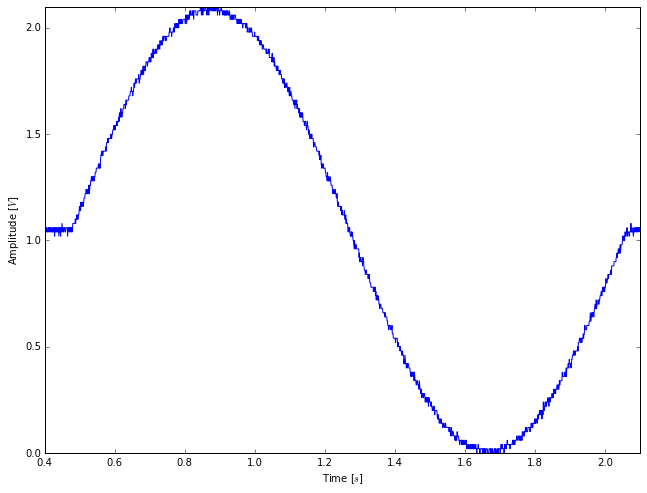
\includegraphics[scale=0.5]{src/Sinus.png}
\caption{Generierter Sinus}
\label{fig:SINUS}
\end{figure}

\begin{figure}[H]
\centering\small
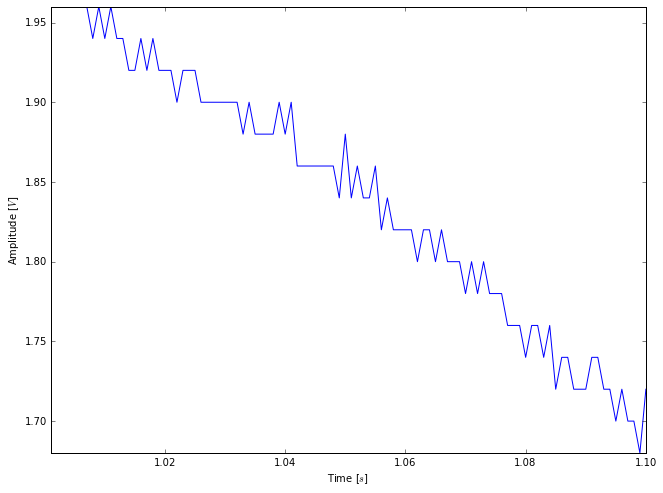
\includegraphics[scale=0.5]{src/Sinus_Ausschnitt.png}
\caption{Sinus Ausschnitt}
\label{fig:SINUS_A}
\end{figure}

\section{Auswertung}
\label{chap:VERSUCH_3_AUSWERTUNG}
In dem Ausschnitt des Sinus (Abbildung \ref{fig:SINUS_A}) sind nun die einzelnen Stufen zu erkennen. Da das Signal Spannungsschwankungen aufweißt, ist es schwer, einen Stufenübergang eindeutig zu bestimmen. Durch ablesen bzw. Vermessen der Dauer der Stufen ergibt sich somit ein mittleres $\Delta t$ von ungefähr $10ms$ und damit eine Frequenz von ca. 100 Hz.
Die Zeit $\Delta t$ variiert ein wenig von Stufe zu Stufe.

\section{Interpretation}
\label{chap:VERSUCH_3_INTERPRETATION}
Da ein Sinus Signal mit einer Sample Rate von 100 Hz auf die Karte des DA-Wandlers geschrieben wurde, war zu erwarten, dass die einzelnen Stufen bzw. Samples auch in diesem Zeit-Bereich liegen.
Es wurden aber auch leichte Abweichungen (Jitter) festgestellt, was zeigt, dass die DA-Wandlung nicht optimal ist.

Auffallend ist auch, dass das komplette Sinus Signal eine Dauer von 1.6 Sekunden aufweist.
Eigentlich müsste das Signal genau eine Sekunde lang sein (Sinus mit 1 Hz), weil wir 100 Sinus-Werte mit einer Sample Rate von 100 Hz auf die Karte schreiben.
Das könnte daran liegen, dass der DA-Wandler maximal 100 Samples pro Sekunde ausgeben kann und wir somit genau an der Grenzfrequenz liegen. Dadurch kommt der DA-Wandler eventuell nicht ''hinterher'' und ist ab und zu langsamer.

%
% CHAPTER Versuch 4
%
\chapter{Versuch 4 - Abtasttheorem}
\label{chap:VERSUCH_4}

Dieser Versuch zeigt, was passiert, wenn man das Abtasttheorem nicht einhält und ignoriert.
Anhand von diversen Sinus Signalen wird dies untersucht.

\section{Fragestellung, Messprinzip, Aufbau, Messmittel}
\label{chap:VERSUCH_4_FRAGESTELLUNG}

Es soll geklärt werden, welche Auswirkungen und welche Bedeutung das Abtasttheorem für die AD-Wandlung hat.
Dafür werden mit einem externen Sinusgenerator 8 Signale erzeugt.
Diese Unterscheiden sich in ihrer Frequenz. Beginnend mit 1000 Hz wird die Frequenz in 1000 Hz Schritten erhöht, bis eine Frequenz von 8000 Hz erreicht ist.
Der AD-Wandler nimmt diese Signale auf und mit dem Programm (Listing \ref{lst:Code}) werden sie abgespeichert und verarbeitet.

\section{Messwerte}
\label{chap:VERSUCH_4_MESSWERTE}

Folgend sind die Spektren aller erzeugten Signale abgebildet.
Abbildung \ref{fig:8000_TIME} zeigt zusätzlich den zeitlichen Verlauf des erzeugten Signals mit 8000 Hz.

\begin{figure}[H]
\centering\small
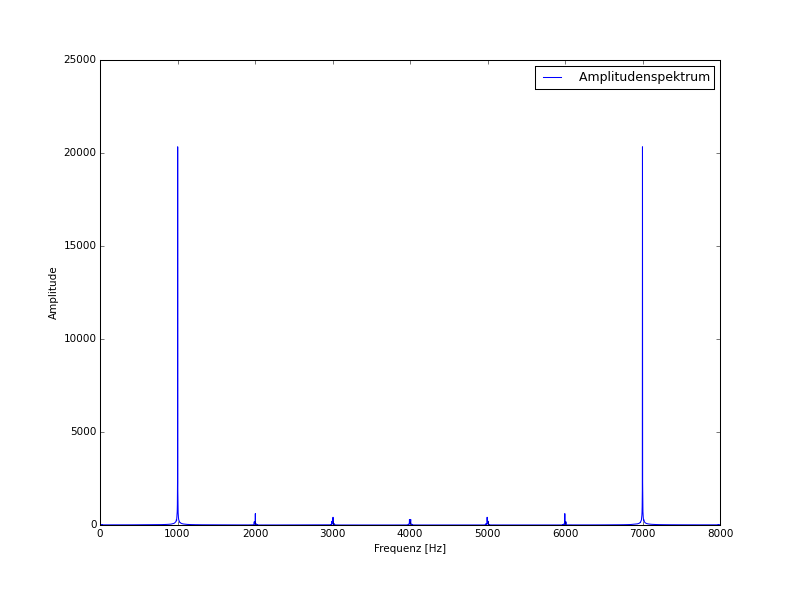
\includegraphics[scale=0.4]{src/1000fft.png}
\caption{Spektrum Sinus mit 1000 Hz}
\label{fig:1000_FFT}
\end{figure}

\begin{figure}[H]
\centering\small
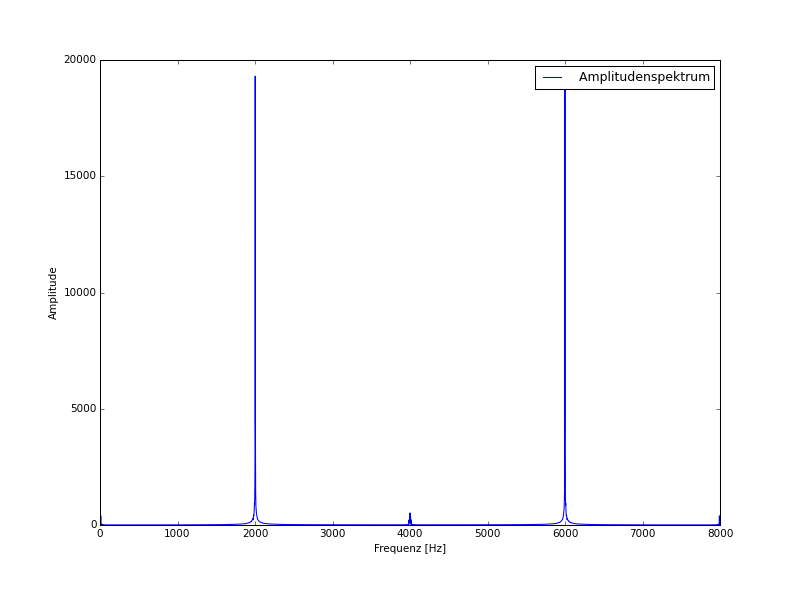
\includegraphics[scale=0.4]{src/2000fft.png}
\caption{Spektrum Sinus mit 2000 Hz}
\label{fig:2000_FFT}
\end{figure}

\begin{figure}[H]
\centering\small
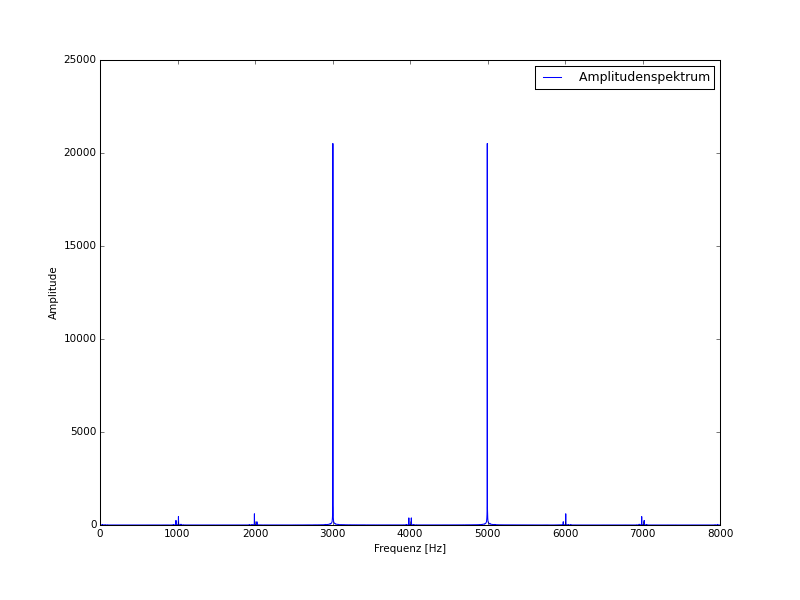
\includegraphics[scale=0.4]{src/3000fft.png}
\caption{Spektrum Sinus mit 3000 Hz}
\label{fig:3000_FFT}
\end{figure}

\begin{figure}[H]
\centering\small
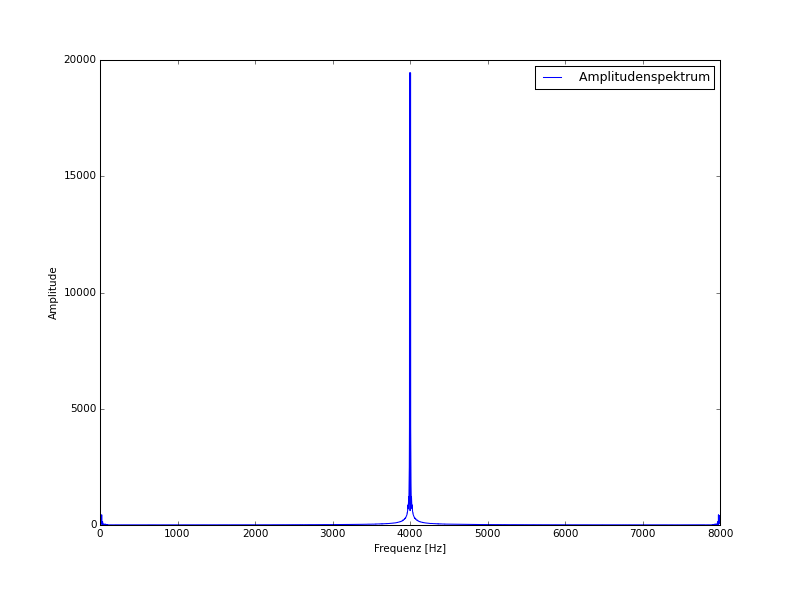
\includegraphics[scale=0.4]{src/4000fft.png}
\caption{Spektrum Sinus mit 4000 Hz}
\label{fig:4000_FFT}
\end{figure}

\begin{figure}[H]
\centering\small
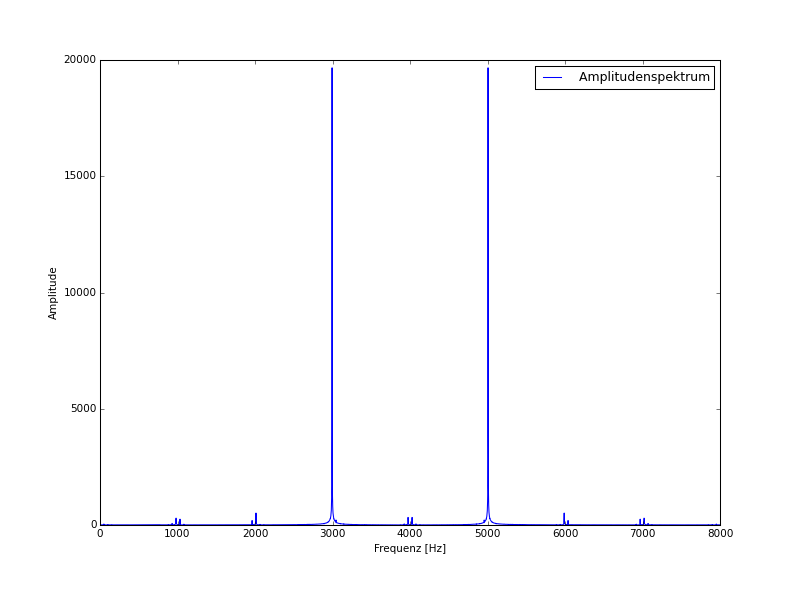
\includegraphics[scale=0.4]{src/5000fft.png}
\caption{Spektrum Sinus mit 5000 Hz}
\label{fig:5000_FFT}
\end{figure}

\begin{figure}[H]
\centering\small
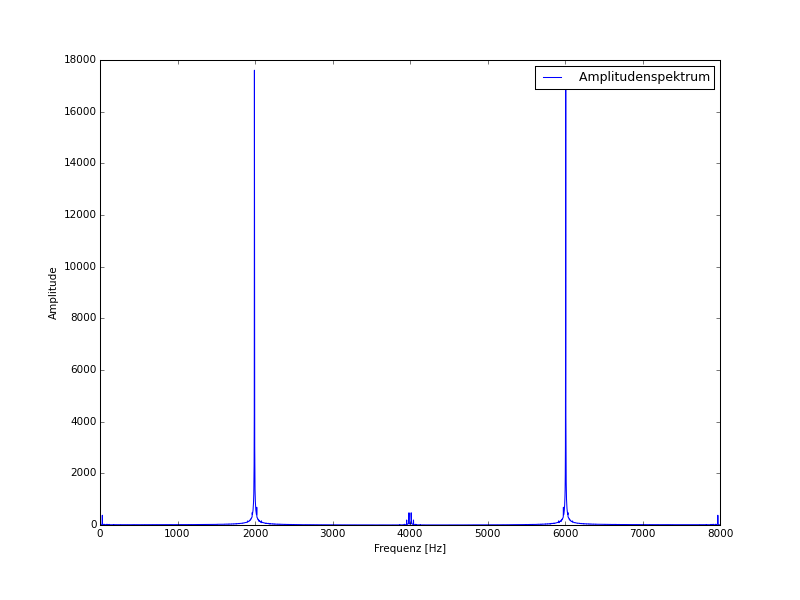
\includegraphics[scale=0.4]{src/6000fft.png}
\caption{Spektrum Sinus mit 6000 Hz}
\label{fig:6000_FFT}
\end{figure}

\begin{figure}[H]
\centering\small
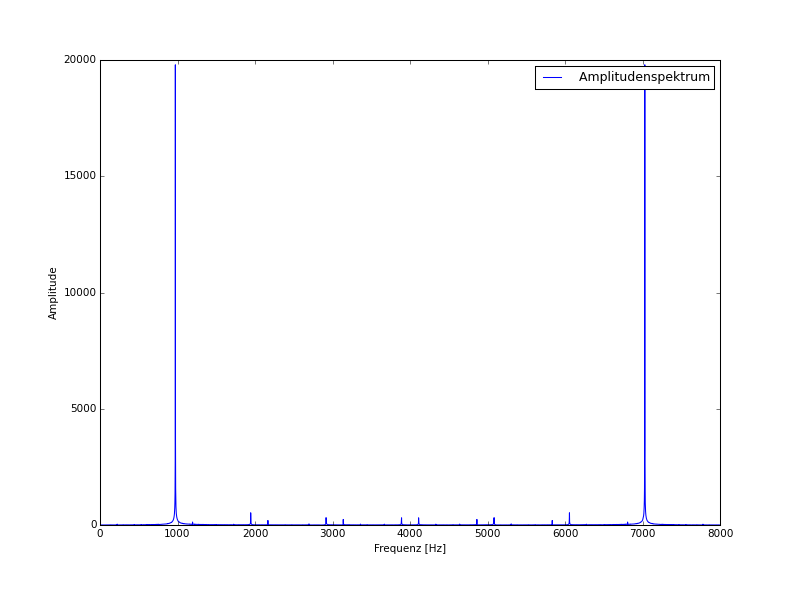
\includegraphics[scale=0.4]{src/7000fft.png}
\caption{Spektrum Sinus mit 7000 Hz}
\label{fig:7000_FFT}
\end{figure}

\begin{figure}[H]
\centering\small
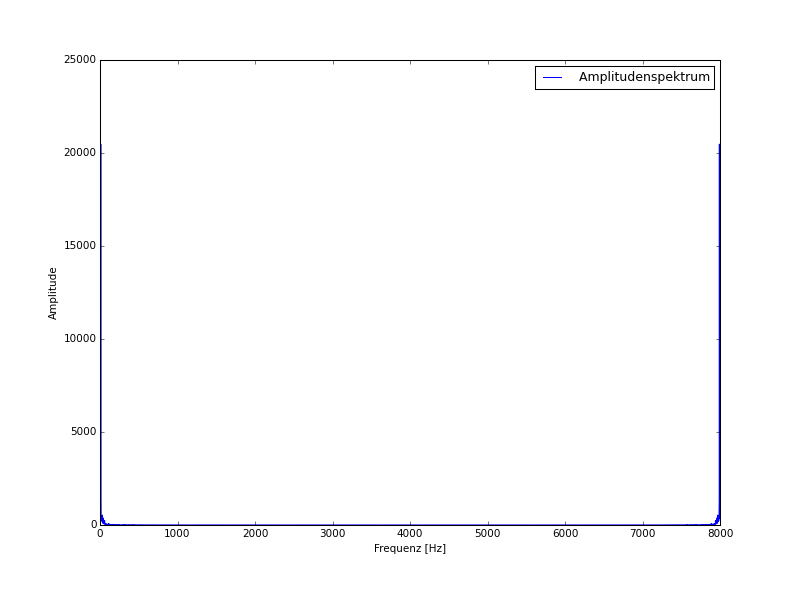
\includegraphics[scale=0.4]{src/8000fft.png}
\caption{Spektrum Sinus mit 8000 Hz}
\label{fig:8000_FFT}
\end{figure}

\begin{figure}[H]
\centering\small
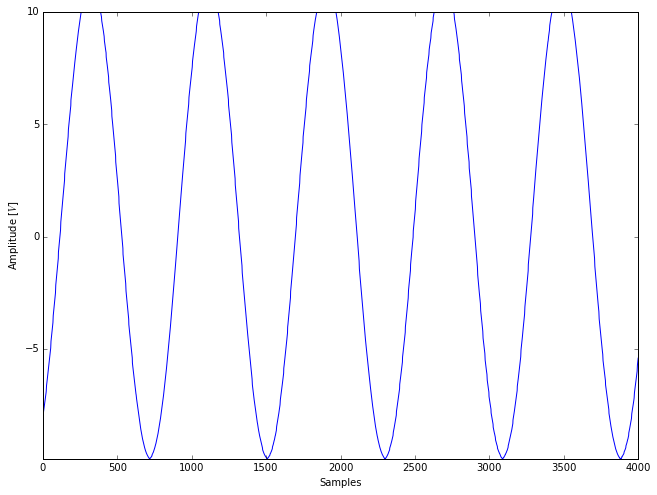
\includegraphics[scale=0.4]{src/Sinus8000Hz.png}
\caption{Zeitverlauf Sinus 8000 Hz}
\label{fig:8000_TIME}
\end{figure}

\section{Auswertung}
\label{chap:VERSUCH_4_AUSWERTUNG}

Da der AD-Wandler eine Abtastfrequenz von 8000 Hz besitzt, liegt die Nyquist-Frequenz bei der Hälfte, also 4000 Hz.
Das Abtasttheorem besagt nun, das die maximal vorkommende Frequenz im abgetasteten Signal nicht größer als die Nyquist-Frequenz sein darf, um das Signal verlustfrei rekonstruieren zu können. D.h. es sollten in diesem Fall nur Frequenzen mit höchstens 4000 Hz aufgenommen werden.

\section{Interpretation}
\label{chap:VERSUCH_4_INTERPRETATION}

Die aufgenommenen Spektren zeigen nun sehr schön, dass sich ab der Nyquist-Frequenz die beiden Peeks ''überholen''.
Man würde dadurch beispielsweise denken, dass die Frequenz des Signals mit 6000 Hz (Abbildung \ref{fig:6000_FFT}) 2000 Hz beträgt, in Wahrheit liegt sie jedoch bei 6000 Hz.
Dieser Fehler gilt für alle Frequenzen über der Nyquist-Frequenz.
Im zeitlichen Verlauf in Abbildung \ref{fig:8000_TIME} kann man erkennen, dass das aufgenommene Signal keineswegs 8000 Hz beträgt, wie es eigentlich sein sollte. Stattdessen liegt die Frequenz des Sinus bei ca. 10 Hz.
Anmerkung: Eigentlich müssten es 0 Hz sein, aber aufgrund von Ungenauigkeiten entsteht dieser Wert.

Offensichtlich führt das Überschreiten der Nyquist-Frequenz zu einer Fehlinterpretation des Signals (Spektrums). Dadurch werden Frequenzen ermittelt bzw. hinzugefügt, welche in dem originalen Signal gar nicht vorgekommen sind.

%
% CHAPTER Anhang
%
\renewcommand\thesection{A.\arabic{section}}
\renewcommand\thesubsection{\thesection.\arabic{subsection}}

\chapter*{Anhang}
\label{chap:APPENDIX}
\addcontentsline{toc}{chapter}{Anhang}
%\setcounter{chapter}{0}
\addtocounter{chapter}{1}
\setcounter{section}{0}

\section{Quellcode für Versuche 1 - 4}
\label{chap:APPENDIX_SOURCECODE}
\begin{lstlisting}[style=PYTHON, frame=single, caption=QuellCodeV1 bis V4, captionpos=b, label=lst:Code]

# -*- coding: utf-8 -*-
"""
Created on Mon Jan 11 14:15:07 2016

@author: edc07
"""


import numpy as np
import matplotlib.pyplot as plt

import redlab as rl
import time
from TekTDS2000 import *


def versuch1():
    out(1)
    #print(str(get_input(4000, 8000)))
    print('fertig')


def versuch2():
    #print(str(np.mean(get_input(4000, 8000))))

    mult_array = np.array([0.103, 0.196, 0.2, 0.2, 0.194, 0.198, 0.199, 0.199, 0.2, 0.198])
    ad_array = np.array([0.015, 0.018, 0.013, 0.015, 0.016, 0.013, 0.012, 0.012, 0.014, 0.022])
    print("Multimeter Philips Std s={}".format(getStd(mult_array)))
    print("AD Wandler Std s={}".format(getStd(ad_array)))

def versuch3():
    da_array = np.array([0.011, 0.019, 0.027, 0.041, 0.049, 0.058, 0.072, 0.080, 0.090, 0.096])
    print("DA Wandler Std s={}".format(getStd(da_array)))

def versuch4():    
    for x in get_sin():
       out(x)
        time.sleep(0.01)
    
    save_input_oszi()
    print(getInputData('sinus.csv')[0])
    
    plotRecord(getInputData('sinus.csv'))


def versuch5():
    np.savetxt('8000.csv', rl.cbVInScan(0, 0, 0, 4000, 8000, 1))
    
    plotFFT(getInputData('1000.csv'), 8000,'1000fft.png')
    plotFFT(getInputData('2000.csv'), 8000,'2000fft.png')
    plotFFT(getInputData('3000.csv'), 8000,'3000fft.png')
    plotFFT(getInputData('4000.csv'), 8000,'4000fft.png')
    plotFFT(getInputData('5000.csv'), 8000,'5000fft.png')
    plotFFT(getInputData('6000.csv'), 8000,'6000fft.png')
    plotFFT(getInputData('7000.csv'), 8000,'7000fft.png')
    plotFFT(getInputData('8000.csv'), 8000,'8000fft.png')


def plotFFT(rec, sampleRate, filename=''):
    
    #fft
    # n = Anzahl der Schwingungen innerhalb der gesamten Signaldauer
    c = np.fft.fft(rec)
    n = np.abs(c)
    sampleTime = 1 / sampleRate
    
    count = np.arange(0, len(n))* (1 / (len(n) * sampleTime))
    
    # Anzahl der Schwingungen innerhalb der gesamten Signaldauer dargestellt
    dpi=75
    fig, axN = plt.subplots(figsize=(800/dpi,600/dpi), dpi=dpi)
    axN.plot(count[:],n[:], color = "blue", label=" Amplitudenspektrum ")
    # lässt X-Achse bei 0 beginnen
    axN.autoscale(enable=True, axis='x', tight=True)
    axN.legend(loc='upper right');
    axN.set_xlabel("Frequenz [Hz]")
    axN.set_ylabel("Amplitude")
    
    # als png abspeichern    
    if filename is not '':
        fig.savefig(filename, transparent=True, dpi=dpi)
    return


def getStd(e_array):
    return np.std(e_array)

def plotRecord(rec):
    myDpi = 75
    fig, ax = plt.subplots(figsize=(800/myDpi, 600/myDpi), dpi=myDpi)
    ax.autoscale(enable=True, axis='x', tight=True)
    ax.plot(rec[400:2100,0], rec[400:2100,1])
    ax.set_xlabel('Time [$s$]')
    ax.set_ylabel('Amplitude [$V$]')


def save_input_oszi():
    scope = TekTDS2000()

    x,y = scope.getData(1,1,2500)
    np.savetxt("sinus.csv" , np.transpose([x,y]), delimiter=",")


def getInputData(filename):
    return np.genfromtxt(filename, delimiter=',')


def get_input(number, samplerate):
    return rl.cbVInScan(0, 0, 0, number, samplerate, 1)


def out(voltage):
    rl.cbVOut(0, 0, 101, voltage)


def get_sin(fs=100):
    val = np.linspace(0, 2 * np.pi, fs)
    return np.sin(val) + 1


def main():
    versuch1()
    versuch2()
    versuch3()
    versuch4()
    versuch5()

if __name__ == '__main__':
    main()
\end{lstlisting}

\section{Messergebnisse}
\label{chap:APPENDIX_MEASUREMENT_SOURCE}

\begin{figure}[H]
\centering\small
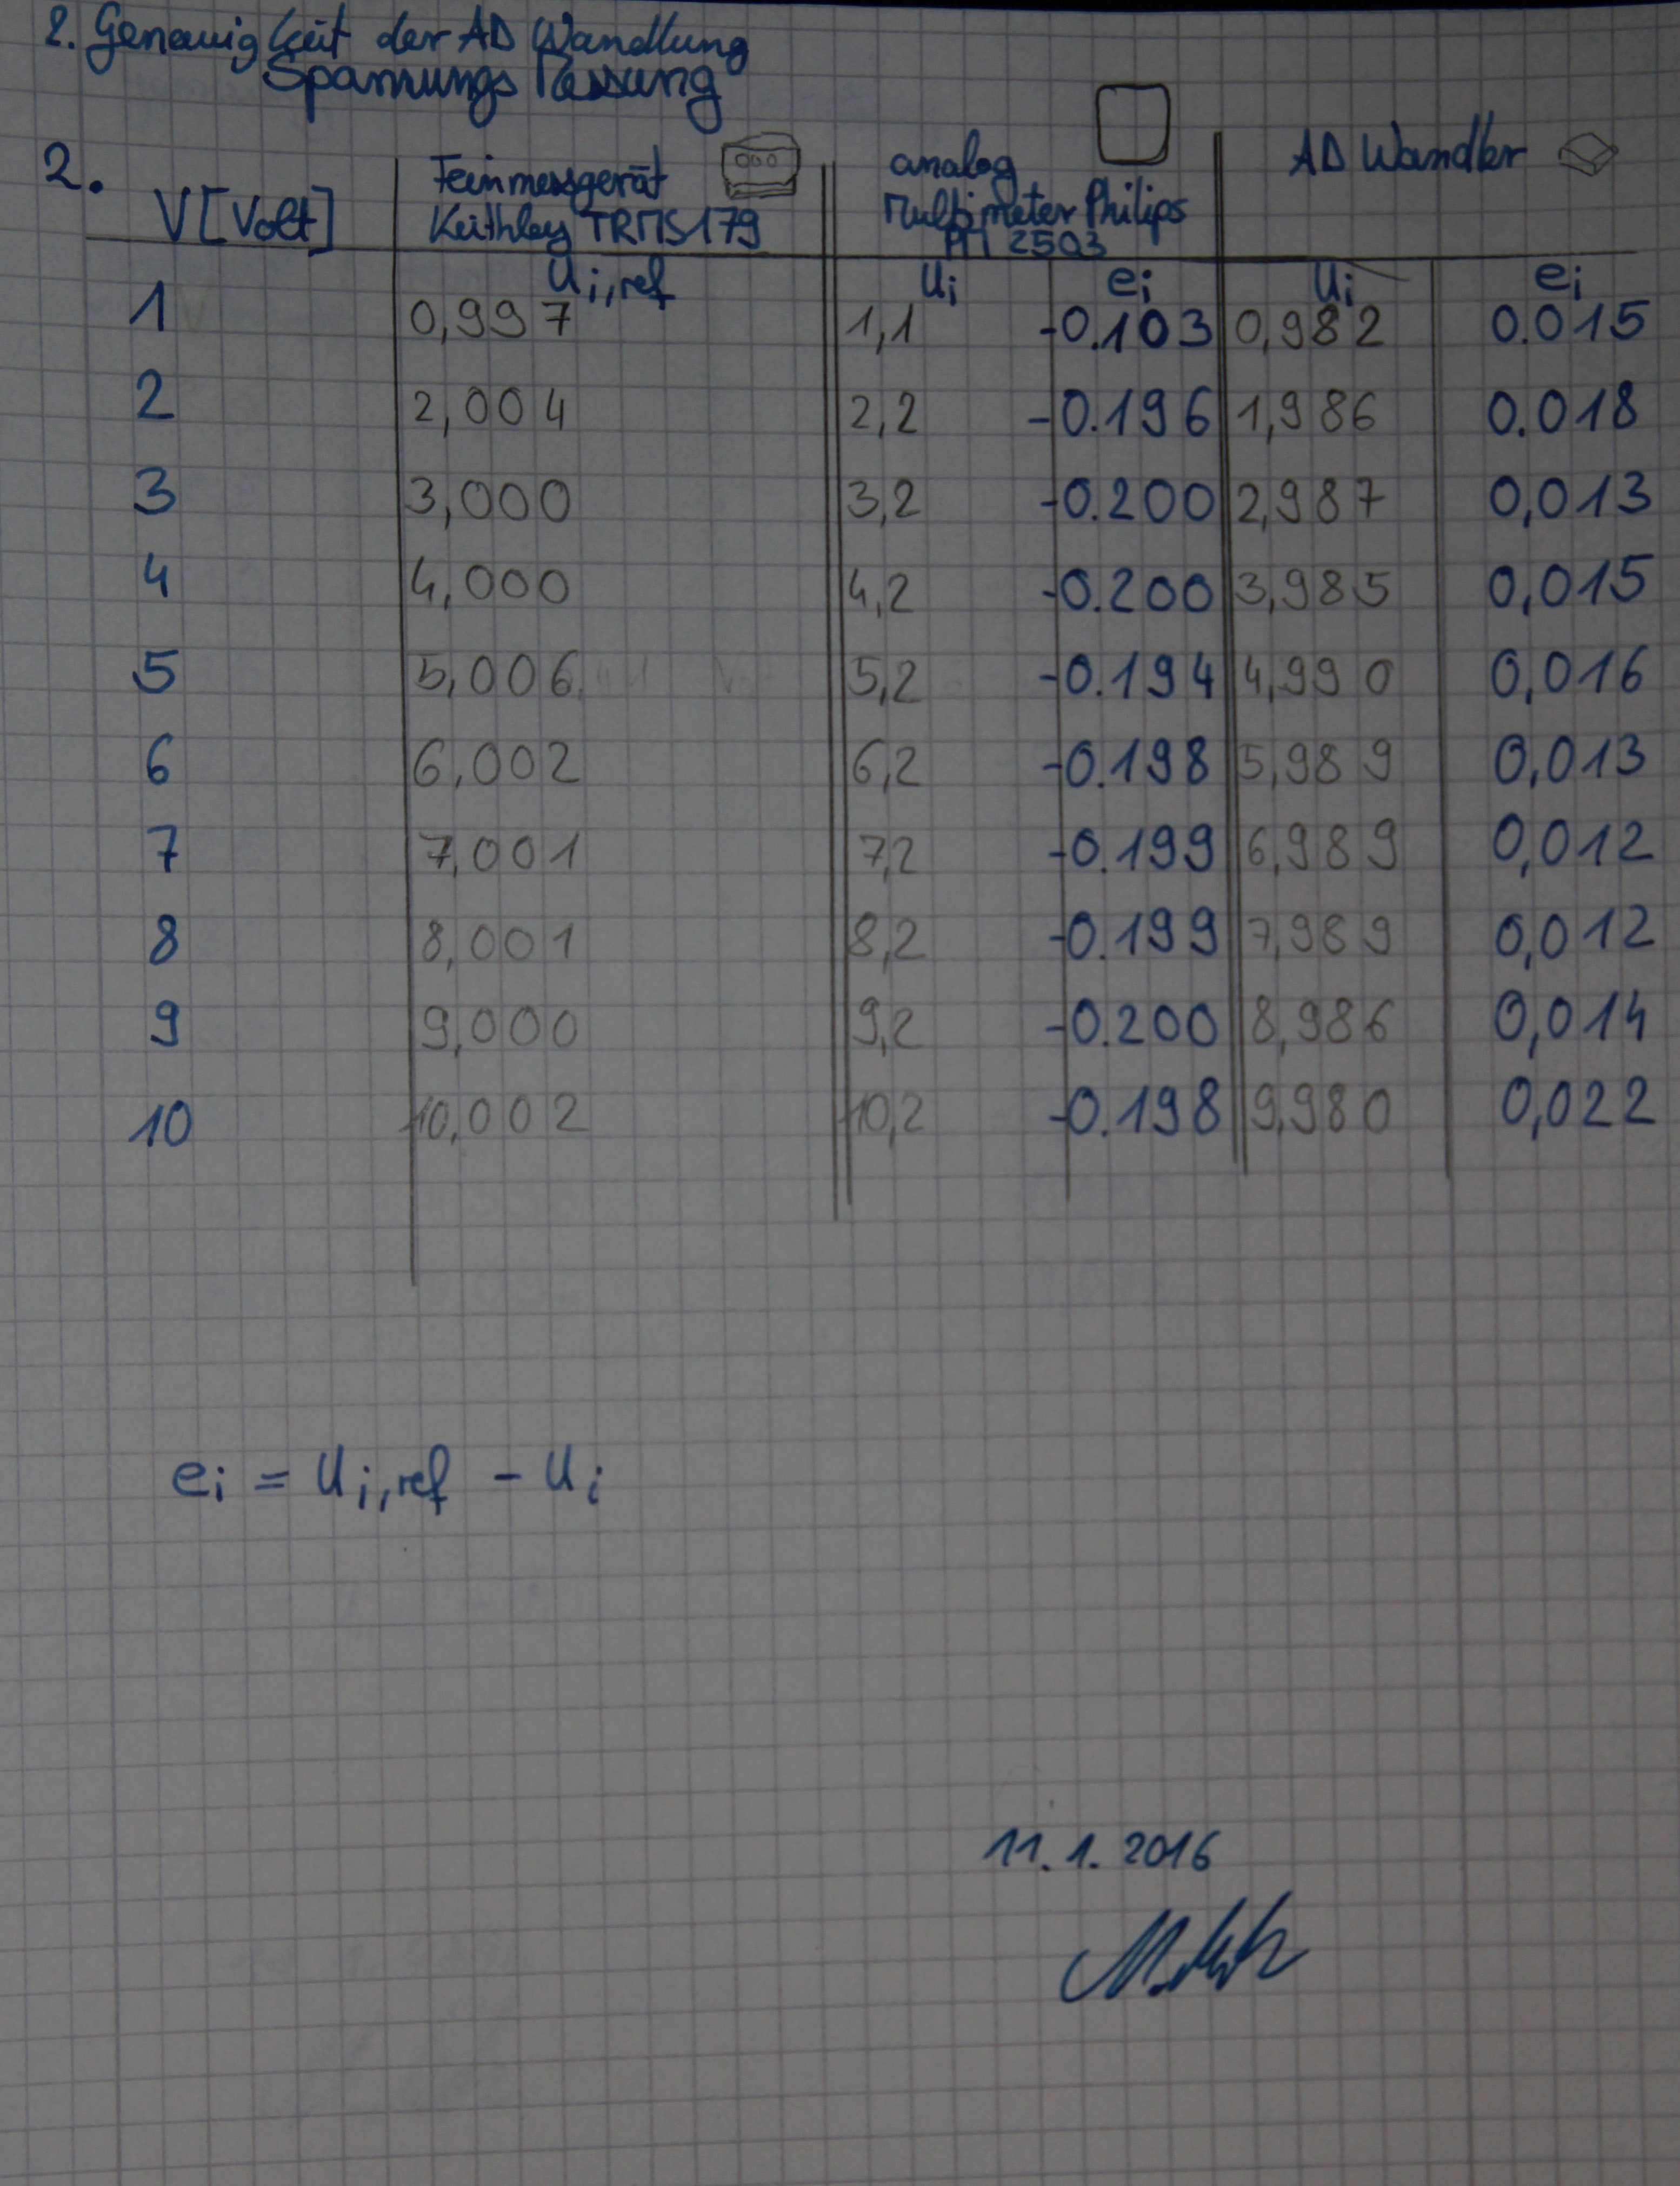
\includegraphics[width=\textwidth]{src/2GenauigkeitsWerteAD.jpg}
\caption{Genauigkeitswerte der AD Wandlung}
\label{fig:AD_WERTE}
\end{figure}

\begin{figure}[H]
\centering\small
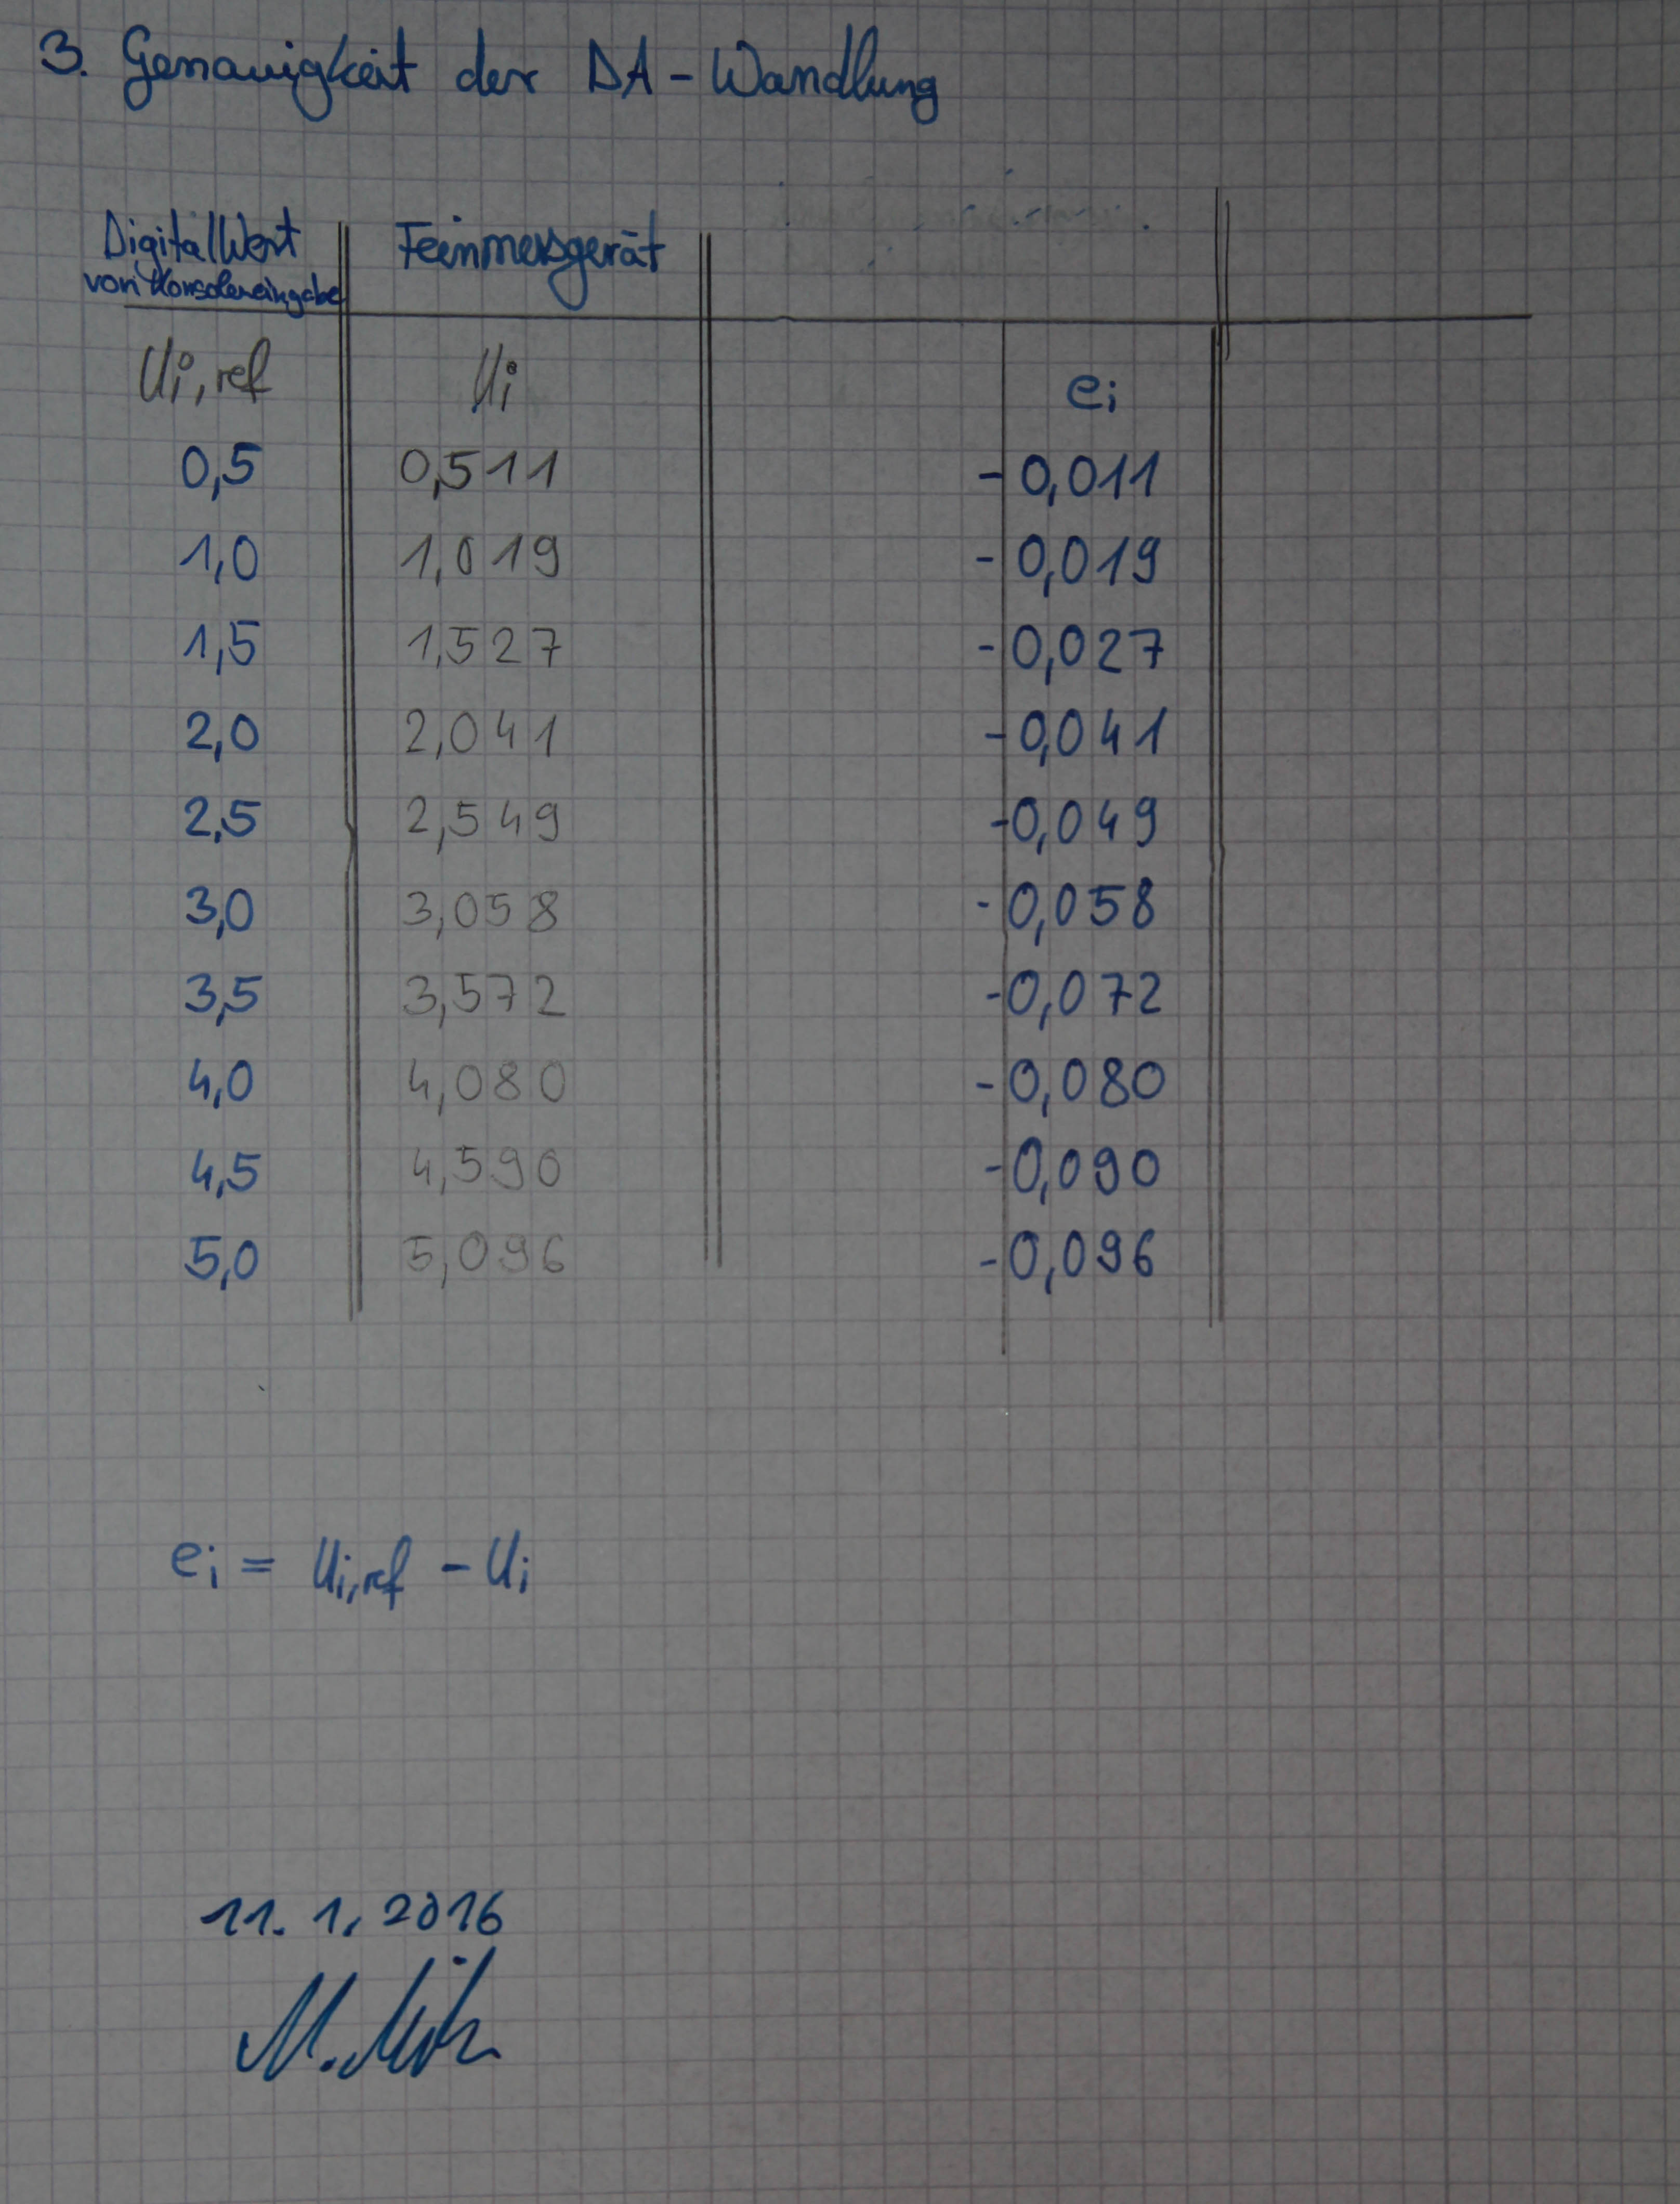
\includegraphics[width=\textwidth]{src/3GenauigkeitsWerteDA.jpg}
\caption{Genauigkeitswerte der DA Wandlung}
\label{fig:DA_WERTE}
\end{figure}

%
% Literaturverzeichnis
%
%
% Literaturverzeichnis
%
\phantomsection
\addcontentsline{toc}{chapter}{Literaturverzeichnis}
\bibliography{../references}
\newpage

\end{document}
%------------------------------------
% ╔═╗╔╗╔╔╦╗  ╔╦╗╔═╗╔═╗╦ ╦╔╦╗╔═╗╔╗╔╔╦╗
% ║╣ ║║║ ║║   ║║║ ║║  ║ ║║║║║╣ ║║║ ║ 
% ╚═╝╝╚╝═╩╝  ═╩╝╚═╝╚═╝╚═╝╩ ╩╚═╝╝╚╝ ╩ 
%------------------------------------